\documentclass{article}
\usepackage[utf8]{inputenc}
\usepackage[T1]{fontenc}
\usepackage{graphicx}
\usepackage{geometry}
\geometry{a4paper}
\usepackage[frenchb]{babel}
\title{Second Harmonic Generation at 952nm}
\author{Xiaoyu Jiang}
\date{12/05/2017}
\begin{document}
\maketitle
\section{Introduction}
We are using a Lithium Tri-Borate(LBO) crystal for a 952nm-476nm Second-Harmonic Generation. Compared to PPKTP crystals, LBOs have lesss blue light absorption, making it insensitive to thermal effect in SHG cavities. The index of refration of LBO crystal at 952nm is 1.608. The front and back surfaces of the crystal are Brewster-cut to minimize reflection loss.
\section{Critical phase-matching}
For SHG in a LBO crystal, critical phase matching is needed. First of all we can use Sellmeier's equation to calculate the index of refractions of 952nm and 476nm lights in LBO(Kato,1994):

$$n_x^2=2.4542+\frac{0.1125}{\lambda^2-0.01135}-0.01388\lambda^2$$

$$n_y^2=2.5390+\frac{0.1277}{\lambda^2-0.01189}-0.01848\lambda^2$$

$$n_x^2=2.4542+\frac{0.1125}{\lambda^2-0.01135}-0.01388\lambda^2$$

However, here we haven't thake temperature in to consideration. For Brewster-cut crystals, the crystal surfaces aren not coated, and in experiments the perfomance of Brewster surfaces will be slowly degraded by air humidity. To prevent this, we decide to head the crystal to about 50 degrees. The temperature-related Sellmeier's equations are(Kato,1994):

$$n_x^2=2.4542+\frac{0.1125}{\lambda^2-0.01135}-0.01388\lambda^2+(-3.76\lambda+2.30)\times10^{-6}\times({\Delta}T+29.13\times10^{-3}({\Delta}T)^2))$$

$$n_y^2=2.5390+\frac{0.1277}{\lambda^2-0.01189}-0.01848\lambda^2+(6.01\lambda-19.40)\times10^{-6}\times({\Delta}T-32.89\times10^{-4}({\Delta}T)^2))$$

$$n_x^2=2.4542+\frac{0.1125}{\lambda^2-0.01135}-0.01388\lambda^2+(1.50\lambda-9.70)\times10^{-6}\times({\Delta}T-74.49\times10^{-4}({\Delta}T)^2))$$

Then using
$${\phi}_m=\arcsin{(\sqrt{\frac{n_{1z}^{-2}-n_{2y}^{-2}}{n_{2x}^{-2}-n_{2y}^{-2}}})}$$
we can get the critical phase-matching angle to be about $18.4^{\circ}$,
\section{Boyd-Kleimann optimization}
\subsection{optimization with a circular waist}
By defining power conversion efficiency $\epsilon=P_2/P_{in}$, we can eventually arrive at the following equation:
$$\sqrt{\epsilon}=\frac{4T\sqrt{E_{NL}P_{in}}}{[2-\sqrt{1-T}(2-L_0-\sqrt{{\epsilon}E_{NL}P_{in}}]^2}$$
in which $T$ is the transmission coefficient, $L_0$ is the additional internal linear loss, and $E_{NL}$ is the crystal conversion efficiency. The conversion efficiency $\epsilon$ can be solved in closed form.

To maxmize the harmonic power, we need to find the optimum configuration for a maximum  $E_{NL}$. According to Boyd-Kleiman theory, the conversion efficiency  $E_{NL}$ satisfies:
$$E_{NL}=\frac{2\omega_1^2d^2}{\pi\epsilon_0c^3n_1^2n_2}\frac{L_c}{w_{10}^2}h$$
Here $omega_1$ is the angular frequency of the fundamental beam, $d$ is the effective susceptibility, $n_1$ and $n_2$ are the corresponding refactive indexes of the fundamental and harmonic beam, $L_c$ is the crystal length, and $w_{10}$ is the waist of the fundamental beam inside the crystal.

h is the Boyd-Kleiman integral, which equals to:
$$h=\int_{\frac{-1}{2}}^{\frac{1}{2}}d\xi^{'}\int_{\frac{-1}{2}}^{\frac{1}{2}}d\xi\frac{e^{i{\Delta}kL_c(\xi-\xi^{'})}}{1+i\frac{L_c}{L_{R1}}\xi}\frac{e^{-\frac{2L_c}{L_{R1}}B^2(\xi-\xi^{'})^2}}{1-i\frac{L_c}{L_{R1}}\xi^{'}}$$

Here $L_{R1}$ is the Rayleigh range of the fundamental Gaussian beam. $L_{R1}={\pi}w_{01}^2/\lambda$

By numerical searching through the expression of $E_{NL}$, we find the optimum $w_{10}$ and ${\Delta}k$. With $w_{10}=34.4{\mu}m$ and ${\Delta}k=119.4m^{-1}$, the maximum $E_{NL}=1.25\times10^{-4}$.

\subsection{optimization with an elliptical waist}
When optimizing conversion efficiency  $E_{NL}$ in the previous section, we are assuming that the waist of the fundamental beam at the center of the crystal should be circular. However this condition does not need to be satisfied. The more general expression for  $E_{NL}$ is:
$$E_{NL}=\frac{2\omega_1^2d^2}{\pi\epsilon_0c^3n_1^2n_2}\frac{L_c}{w_{10t}w_{10s}}h$$
with B-K integral:
$$h=\int_{\frac{-1}{2}}^{\frac{1}{2}}d\xi^{'}\int_{\frac{-1}{2}}^{\frac{1}{2}}d\xi\frac{e^{i{\Delta}kL_c(\xi-\xi^{'})}}{\sqrt{1+i\frac{L_c}{L_{R1t}}\xi}\sqrt{1+i\frac{L_c}{L_{R1s}}\xi}}\frac{e^{-\frac{2L_c}{L_{R1t}}B^2(\xi-\xi^{'})^2}}{\sqrt{1-i\frac{L_c}{L_{R1t}}\xi^{'}}\sqrt{1-i\frac{L_c}{L_{R1s}}\xi^{'}}}$$

Here $L_{R1t}$ and $L_{R1s}$ are the Rayleigh ranges of the fundamental Gaussian beam in the tangential and sagittal plane. $L_{R1t}={\pi}w_{01t}^2/\lambda$, $L_{R1s}={\pi}w_{01s}^2/\lambda$. $w_{01t}$ and $w_{01s}$ are the tangential and sagittal waist at the center of the crystal , respectively.

By numerical searching the B-K optimal waists are $w_{01t}=52.2{\mu}m, w_{01s}=24.0{\mu}m$, with ${\Delta}k=117m^{-1}$. $E_{NL}=1.48\times10^{-4}$. 

Although the optimal waists might not be achievable, we can make the beam waist slightly elliptical based on the circular-waist design, which would increase the conversion efficiency. By assuming that ${w_{01t}}/{w_{01s}}=5/4$, we can find the B-K optimal waists: $w_{01t}=39.846{\mu}m, w_{01s}=31.8768{\mu}m$, with ${\Delta}k=112.899m^{-1}$. $E_{NL}=1.42\times10^{-4}$. 

\section{cavity design}
We are using a bow-tie cavity with two flat mirrors and two curved mirrors to enhace the efficiency of the harmonic generation. The sketch of the cavity is shown as follow:

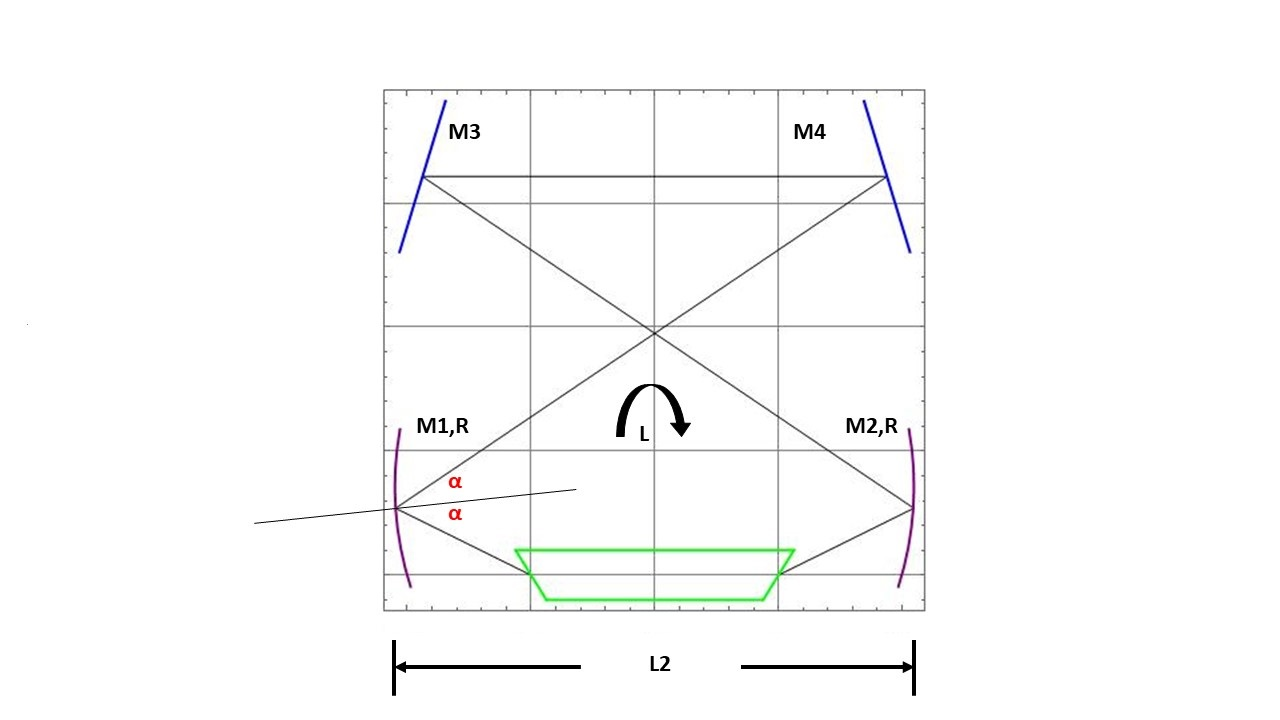
\includegraphics[height=3in]{bcut1.JPG}

Assuming that the two curved mirrors has the same radius of curvature, then in the cavity design we have 4 free parameters: round trip length $L$, seperation between curved mirrors $L_2$, mirror incidence angle $\alpha$, and radius of curvature of the mirrors $R$. These parameters need to meet the following requirements: the tangential and sagittal waist of the beam must be equal at the center of the crystal; the size of the waist should equal to the B-K optimum waist calculated in section 3. 

For a bow-tie cavity with Brewster cut crystals, we can see that the beam reflecting on the curved mirrors are off-axes beams. The incidence angle $\alpha$ cannot be zero. Then as a result, the off-axes beams will bring abberations, thus degrading the focus and increasing the linear loss in the cavity. It can be noticed that when refracting on Brewster surfaces, such distortion will also occure. To compensate for abberations like coma and astigmatism, we can carefully choose $\alpha$ and $R$ to make the mirror-induced abberations and crystal-induced abberations cancel with each other. 
According to Dunn and Ferguson,1977, (It seems that one the equations in J.S.Nielsen, 1994 is wrong?) the optimum $\alpha$ and $R$ are:
$$\alpha=\arctan{(\frac{n^3}{2(n^2+1)})}$$
$$R=\frac{2L_c(n^4-1)(n^2+1)^{1/2}}{\sin{(\alpha)}n^7}$$
which in our case, $\alpha=30.1^{\circ}$, $R=3.1cm$.

Then we choose $L$ and $L_2$ to make the tangential and sagittal waist match the B-K optimium waist at the crystal center. We get $L=16.6cm$, $L_2=4.65cm$.

The following figure shows the tangential waist and sagittal waist at the center of the crystal, with respect to the value of $L_2$:

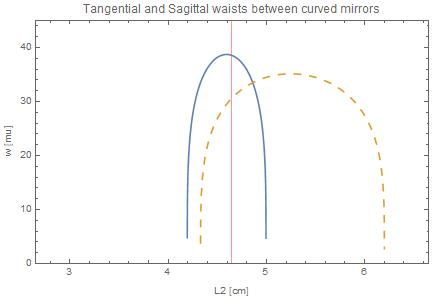
\includegraphics[height=2in]{bcutel1.JPG}

Cavity picture:

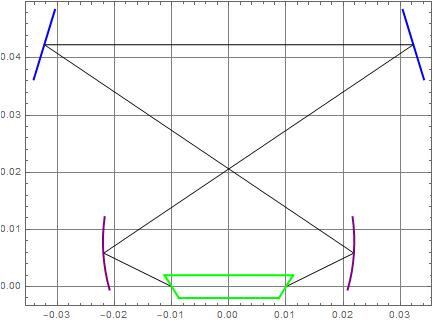
\includegraphics[height=3in]{bcutel2.JPG}

\section{Intracavity Conversion Efficiency}
As defined int the previous section, the power conversion efficiency $\epsilon=P_2/P_{in}$ follows:
$$\sqrt{\epsilon}=\frac{4T\sqrt{E_{NL}P_{in}}}{[2-\sqrt{1-T}(2-L_0-\sqrt{{\epsilon}E_{NL}P_{in}}]^2}$$

For different linear losses and transmission coefficients, we can make plots of the cavity output power:

\end{document}

%------------------------------------------------------------------------------------------------------------------